\documentclass[10pt,twocolumn,letterpaper]{article}
\usepackage[review,datasets]{wacv}
\usepackage{times}
\usepackage{epsfig}
\usepackage{graphicx}
\usepackage{amsmath}
\usepackage{amssymb}
\usepackage{booktabs}
\usepackage[pagebackref,breaklinks,colorlinks]{hyperref}

\def\wacvPaperID{3638}
\def\confName{WACV}
\def\confYear{2027}
\newcommand{\publicCodeURL}{camera-ready repository URL}
\newcommand{\anonymousCodeURL}{anonymous review repository URL}

\newcommand{\kap}{\kappa}
% the crop-read weighting, reported beside the source-pixel one
\newcommand{\kapcr}{\kappa_{\mathrm{cr}}}
\newcommand{\A}{\mathcal{A}}

\begin{document}

\title{Crop-Label Alignment: Auditing Crop-Dependent\\Auto-Labels in Remote-Sensing
Segmentation\\\vspace{4pt}\Large Supplementary Material}
\author{Anonymous \confName{} Datasets Track submission\\Paper ID \wacvPaperID}
\maketitle

\paragraph{Review artifact.}
\iftoggle{wacvfinal}{The public repository is available at
\url{\publicCodeURL}.}{The submitted code and compact evidence package are shared
through an anonymous review repository. Public author-identifying URLs are withheld
from this supplementary PDF during double-blind review.}

\section{Splits, units and what is held fixed}

\paragraph{Sea ice.} 169{,}051 patches of $128 \times 128$ pixels over 39 tiles and
17 acquisitions, each patch centred on an ICESat-2 token, drawn as a
class-stratified subsample of 10{,}000 tokens per acquisition from three strong
beams. Coverage is uneven by construction: the artefact set is a strip along the
satellite track, and a source pixel is covered by between 1 and over 100 patches.
Folds are leave-one-acquisition-out. Model selection uses the first two acquisitions
in sorted order, which is the same pair for most folds and never includes the
held-out one.

\paragraph{Floods.} Sen1Floods11~\cite{bonafilia2020sen1floods11} has 446 chips of $512 \times 512$ pixels over 11 events. The crop
sweep takes $128 \times 128$ crops on a stride-32 grid, $13 \times 13 = 169$
positions per chip, drawing 24 per chip per epoch during training and evaluating
$\kap$ on all 169. Folds are leave-one-event-out, model selection holds out a second
whole event, and normalisation statistics are computed from that fold's training
chips only.

\paragraph{The comparison.} The primary conclusions use contrasts between arms with
the same imagery, crop grid, architecture and sampling order under a fixed training
seed. Raw arm values are also reported to expose the control floor. What varies is
the training-label construction.

\paragraph{How the arms are built.} Every arm is an explicit field of per-crop
thresholds, one value for each of the $169$ crop positions in each of the 446 chips,
written to disk before any training. The dial arms interpolate between the published
per-event constant and a predominantly per-crop Otsu field. Of 75{,}374 positions,
72{,}029 are direct crop fits (95.56\%), 2{,}331 use a finite chip fallback
(3.09\%), and 1{,}014 in six chips remain unusable (1.35\%). Arrays span all 446
chips; training, scoring and arm summaries use the common 440-chip set. The \emph{scramble}
arm randomly permutes threshold positions within each chip. The multiset of
thresholds inside a chip is unchanged, which the builder asserts by sorting both and
comparing. Over the full serialized 446-chip mapping (including the six excluded
rows), 461 assignments (0.61\%) are fixed points, 21.78\% pair overlapping donor
and recipient crops, and every donor shares the same chip. Mean threshold and
within-chip spread are identical to the per-crop arm at $-17.796$\,dB and
$1.453$\,dB. The \emph{offset} arm adds one $N(0, 1.453)$ draw per chip to the
published constant, so it varies between chips at the same scale and not within them.
The scramble attenuates but does not remove the threshold--input correspondence; the
offset is crop-invariant within each chip.

\paragraph{Aggregation.} In the flood arms, seeds are averaged within an event
before anything else, because the event is the held-out evaluation unit. A held-out
fold is not an independent replicate: the eleven models are leave-one-event-out folds sharing nearly all of
their training data, which is why neither benchmark's fold summary carries a test.

\paragraph{Per-fold sea-ice results.} \Cref{tab:perfold} gives the sea-ice result
one acquisition at a time, treated arm against its matched control on identical
pixels, so the aggregate the main paper reports can be read against its parts.

\begin{table}[t]
\centering
\scriptsize
\setlength{\tabcolsep}{2.4pt}
\resizebox{\linewidth}{!}{%
\begin{tabular}{lcccccc}
\toprule
acquisition & $\kap$ treated & $\kap$ control & difference & $\Omega$ tr. & $\Omega$ ct. & $|\A|$ \% \\
\midrule
20191103184432 & +0.2019 & +0.0051 & +0.1968 & 0.0573 & 0.0185 & 7.4 \\
20191104195311 & +0.1568 & +0.0025 & +0.1544 & 0.0415 & 0.0171 & 13.1 \\
20191106190152 & +0.1952 & +0.0118 & +0.1833 & 0.0572 & 0.0344 & 12.1 \\
20191111200211 & +0.0413 & +0.0000 & +0.0413 & 0.1454 & 0.0000 & 4.0 \\
20191113191053 & +0.2257 & +0.0155 & +0.2102 & 0.0308 & 0.0227 & 7.5 \\
20191115195353 & +0.1105 & +0.0296 & +0.0809 & 0.0933 & 0.0640 & 23.1 \\
20191116192813 & +0.1759 & +0.0052 & +0.1707 & 0.0465 & 0.0256 & 11.5 \\
20191117190234 & +0.1218 & +0.0066 & +0.1152 & 0.0662 & 0.0396 & 20.4 \\
20191118183654 & +0.0955 & +0.0139 & +0.0816 & 0.1289 & 0.0861 & 27.0 \\
20191119194532 & +0.0632 & +0.0141 & +0.0491 & 0.0496 & 0.0446 & 14.1 \\
20191120191952 & +0.2216 & +0.0031 & +0.2185 & 0.0246 & 0.0114 & 5.9 \\
20191121185413 & +0.1436 & +0.0052 & +0.1384 & 0.0400 & 0.0226 & 10.5 \\
20191122182834 & +0.1327 & +0.0079 & +0.1249 & 0.0523 & 0.0182 & 12.1 \\
20191123180255 & +0.1934 & +0.0104 & +0.1830 & 0.0552 & 0.0398 & 9.5 \\
20191124191133 & +0.1812 & +0.0201 & +0.1611 & 0.0480 & 0.0265 & 7.7 \\
20191126182014 & +0.2301 & +0.0101 & +0.2201 & 0.0302 & 0.0173 & 7.3 \\
20191127175434 & +0.0903 & +0.0048 & +0.0855 & 0.1083 & 0.0461 & 31.6 \\
\midrule
mean & +0.1518 & +0.0097 & +0.1421 & 0.0632 & 0.0314 & 13.2 \\
\bottomrule
\end{tabular}
}
\caption{Every sea-ice fold in the optical-only primary arm (seed 42). The treated
model trains on the per-patch labels, the control on labels regenerated once per
scene, both on identical pixels. The difference column is what the paper reports:
mean +0.1421, descriptive sd 0.0585, positive in 17 of 17 dependent folds. $|\A|$ is
the artefact set as a percentage of covered pixels. The photon-enabled seed-7
sensitivity is reported separately rather than averaged into this table.}
\label{tab:perfold}
\end{table}


\section{The full experimental configuration}

\Cref{tab:setup} gives the complete configuration. Every cell is filled; ``--''
marks a setting that does not apply to that arm.

\begin{table*}[t]
\centering
\footnotesize
\setlength{\tabcolsep}{5pt}
\begin{tabular}{llll}
\toprule
 & \textbf{sea ice} & \textbf{floods, whole chip} & \textbf{floods, crop sweep} \\
\midrule
architecture       & U-Net~\cite{ronneberger2015unet} & U-Net & U-Net \\
encoder            & ResNet-18~\cite{he2016deep} & ResNet-18 & ResNet-18 \\
encoder init       & ImageNet~\cite{deng2009imagenet} & ImageNet & ImageNet \\
optical channels   & 3                    & --                   & -- \\
SAR channels       & --                   & 2 (VV, VH)           & 2 (VV, VH) \\
photon features    & 0 primary; 10 sensitivity & --            & -- \\
crop size          & $128 \times 128$     & $512 \times 512$ (whole chip) & $128 \times 128$, stride 32 \\
\midrule
optimiser          & AdamW~\cite{loshchilov2019decoupled} & AdamW & AdamW \\
learning rate      & 1e-4, cosine over the cap & 3e-4, constant & 3e-4, constant \\
weight decay       & 1e-4                 & 1e-4                 & 1e-4 \\
loss               & focal~\cite{lin2017focal} & cross-entropy & cross-entropy \\
batch size         & 128                  & 8                    & 32 \\
epoch cap          & 12                   & 40                   & 30 \\
early-stop patience & 5                   & 10                   & 8 \\
\midrule
held-out unit      & acquisition          & flood event          & flood event \\
folds              & 17                   & 11                   & 11 \\
seeds              & 42 primary; 7 sensitivity & 42, 7, 123      & 42, 7, 123 \\
\bottomrule
\end{tabular}
\caption{Configuration for the three experimental arms. Every cell is filled;
``--'' marks a setting that does not apply. Model selection is by best validation
mIoU throughout. The sea-ice
primary is seed 42 with the photon branch disabled; seed 7 is photon-enabled and is
a separately reported input-mode sensitivity and is excluded from the primary average. The seven flood
crop-sweep arms use seeds 7, 42 and 123; all three scramble models share one threshold
reassignment.}
\label{tab:setup}
\end{table*}

\section{Limits of fold-level inference}

Neither benchmark provides independent evaluation units for population inference. The 17 sea-ice folds are
overpasses of 39 tiles across 25 days sharing geography and almost all training data;
the eleven flood folds are leave-one-event-out models sharing nearly all of theirs.
We therefore report effect sizes, descriptive standard deviations, per-fold values
and training-seed sensitivity, but no $p$-values, confidence intervals, power
calculations or required sample sizes over folds.

\section{Association with expert-label performance}

Sea ice has no reference labels, so it can show greater own-crop label alignment but
not its relationship to human annotation. Sen1Floods11 has both. Training on each label set and scoring
both against the expert labels on the same held-out event gives a transfer collapse
of $-0.0454$ mIoU (sd $0.0470$), negative in 9 of 11 events. Model input is
Sentinel-1 throughout, since the expert labels
were produced by analysts correcting a Sentinel-2 classification and the reference
arm is open-loop only while the model never reads Sentinel-2.

The collapse is largest where labeller and human disagree most
($r = +0.719$), but this correlation does not identify a mechanism. An
arm scored against expert labels is bounded by the agreement between the label sets,
so that correlation is expected under any hypothesis, and dropping the two extreme
events takes it to $+0.32$. This is an association between algorithmic training
labels and expert-label performance. It does not isolate the contribution of crop
dependence. We report it here because sea ice has no human reference.

This result is supplementary because it does not measure the crop-dependent
artefact directly. Sea ice, where that artefact occurs, has no human reference;
Sen1Floods11 supplies the reference needed to ask the performance question. The
answer therefore applies to this algorithmic-label construction as a whole.

\section{Recovering the flood labeller}

Sen1Floods11 publishes its per-event threshold, so recovery of its labeller can be
checked independently. Reading the raw band and thresholding it
reproduces the published labels on 95.2\% of pixels, but the recovered threshold sits
$1.11$\,dB low on every one of the eleven events. The consistent sign points to a
systematic cause: a smoothing step we had not applied.
\Cref{fig:recovery} sweeps the radius: the bias crosses zero at a $9 \times 9$ focal
mean, where all eleven events land within $0.25$\,dB at $99.08\%$ agreement and the
largest miss is $0.09$\,dB. That is the preprocessing the dial of the main paper
holds fixed while it varies the threshold alone.

\begin{figure}[tb]
\centering
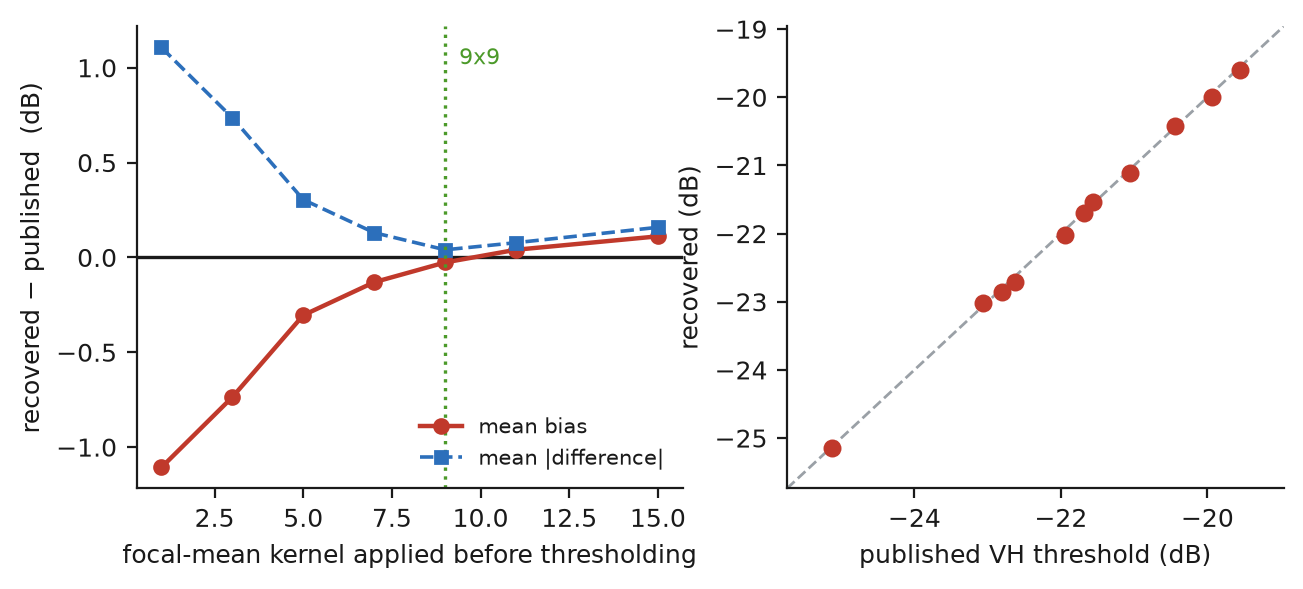
\includegraphics[width=\linewidth]{figures/fig3_generator_recovery.png}
\caption{Left: bias and mean absolute difference against the published thresholds as
the smoothing kernel is swept. Right: recovered against published threshold, one
point per event. The bias crosses zero at a $9 \times 9$ focal mean, where 11 of 11
events land within $0.25$\,dB.}
\label{fig:recovery}
\end{figure}

\section{Stepwise ablation of the published labeller}

\begin{table}[tb]
\centering
\small
\setlength{\tabcolsep}{3pt}
\begin{tabular}{cccc@{\hspace{7pt}}rr}
\toprule
\multicolumn{4}{c}{fitted per crop} & \multicolumn{2}{c}{$P(\A)$} \\
\cmidrule(lr){1-4}\cmidrule(l){5-6}
backgd. & Otsu & norm.\,1 & norm.\,2 & mean & max \\
\midrule
$\bullet$ & $\bullet$ & $\bullet$ & $\bullet$ & $37.04\%$ & $57.90\%$ \\
          & $\bullet$ & $\bullet$ & $\bullet$ & $19.46\%$ & $40.85\%$ \\
$\bullet$ &           & $\bullet$ & $\bullet$ & $26.93\%$ & $47.71\%$ \\
$\bullet$ & $\bullet$ &           & $\bullet$ & $37.04\%$ & $57.90\%$ \\
$\bullet$ & $\bullet$ & $\bullet$ &           & $37.04\%$ & $57.90\%$ \\
          &           & $\bullet$ & $\bullet$ & $4.50\%$  & $40.07\%$ \\
          &           &           &           & $0.00\%$  & $0.00\%$ \\
\bottomrule
\end{tabular}
\caption{The cloud and shadow stage of the released labeller, run per crop on 446
public Sen1Floods11 optical chips, 169 crops each, nothing trained. A dot marks a
quantity estimated from the crop rather than from the whole scene, so the top row is
the pipeline as published. Bands are stacked in the order \texttt{cv2.imread} produces,
which is what the pipeline is fed. Stage 1 alone, which fits nothing, gives $0.00\%$
on every chip.}
\label{tab:published}
\end{table}

The published labeller fits four quantities to whatever array it is handed, and
\cref{tab:published} moves each of them to the scene in turn. Moving the median
background and the Otsu threshold takes $P(\A)$ from $37.04\%$ to $4.50\%$. Moving
either normalisation instead leaves the result bitwise identical.

A min-max is the identity on an array that already spans the range it maps onto, and
with the background and the Otsu threshold fitted per crop that is what it is handed.
The array reaching the first normalisation already spans $0$ to $255$ in $98.7\%$ of
the 75,374 crops, and the array reaching the second already spans the scene's own
second range in $99.0\%$. On the 787 crops where the two ranges genuinely differ, so
the substitution has something to do, we compared the class maps pixel by pixel and
found no pixel changed, for either normalisation. Constant arrays, where the two
branches could diverge because OpenCV maps a constant to zero, occur in 956 crops and
change nothing either.

Repair the background and the Otsu threshold and the array is narrower and varies
between crops, and the normalisations then carry the $4.50\%$ that is left. A step can
be inert beside a larger one and become the whole of what remains once that one is
fixed.

\paragraph{How much of this is our preparation.} Reflectance is scaled to 8 bits by
one global constant, so no per-crop statistic enters before the rule under test.
Thus, a nonzero $P(\A)$ originates in the rule under test. Its magnitude can still
depend on the constant, so we varied that constant. At ceilings of
$2000$, $3000$ and $5000$, which clip $11.5\%$, $3.5\%$ and $0.8\%$ of samples, the
published pipeline reads $35.04\%$, $37.04\%$ and $37.48\%$, and the residual after
repairing the background and the Otsu threshold reads $2.99\%$, $4.50\%$ and $6.18\%$.
The headline is stable and the residual is not, moving by a factor of two across a
range of ceilings that changes the clipped fraction fifteenfold. It stays clearly
nonzero throughout, which is the claim it is asked to carry, and it is not a
quantity to compare across papers.

Repairing the most obvious step may leave an artefact in a later step, and the order
of repairs can change which component appears responsible. The full ablation exposes
that interaction more clearly than a single before-and-after comparison.

\section{A real-image example from the published labeller}

Figure 1 of the main paper is a schematic, so \cref{fig:realmech} is the same
picture built from a Sentinel-2 scene by \texttt{shadow\_cloud}, the published
function, in the two modes the ablation above uses. We train no model and introduce
no learned parameters beyond quantities fitted by that routine.

\begin{figure*}[t]
\centering
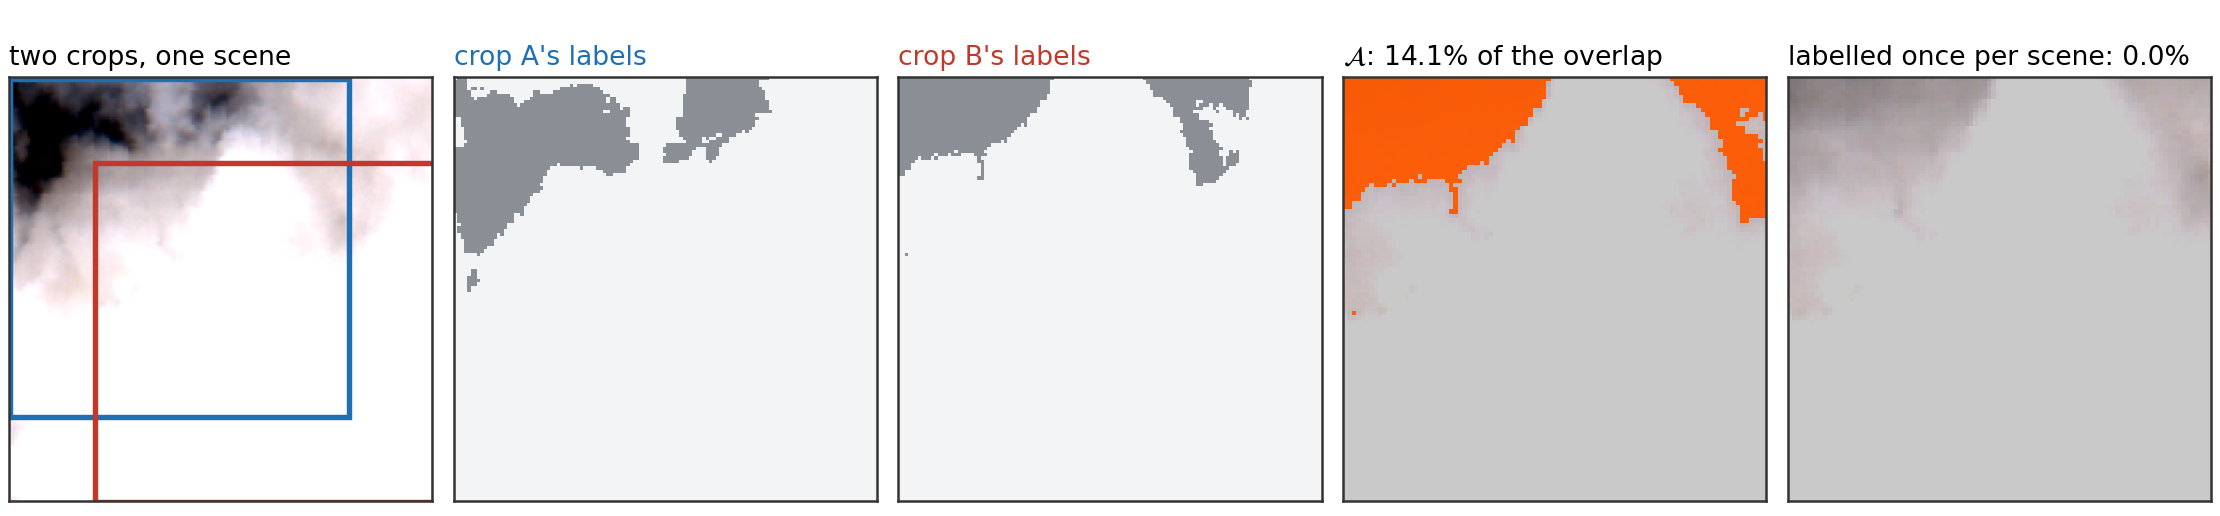
\includegraphics[width=\textwidth]{figures/fig5_mechanism_real.png}
\caption{Two $128 \times 128$ crops 32 pixels apart on one Sentinel-2 region, labelled
by the published cloud and shadow stage. The two crops see the same cloud edge
against different windows, so the Otsu threshold each fits differs and the same
source pixels come out ice in one crop and thin ice in the other: $\A$ is
$14.1\%$ of the overlap and traces the cloud boundary. Fitting the same four
quantities once over the region instead makes the two crops agree everywhere,
and $\A$ is empty. The region was chosen from a scan of 61 sites over 12 scenes,
reported below: 53 of the 61 have a nonempty artefact set, the median is $1.23\%$
and the largest is $38.90\%$, so this example sits above
the median and well below the worst. Contrast is stretched between the 2nd and
98th percentiles of the region for display, which changes no number here.}
\label{fig:realmech}
\end{figure*}

The scan is reproducible as printed: \texttt{fig\_mechanism\_real.py --scan}
with the shipped defaults proposes ten sites in each of twelve scenes at seed 0,
rejects windows crossing swath boundaries, accepts 61, and writes
\texttt{mechanism\_survey.json}. The four numbers above are recomputed from that
file. A single region demonstrates the mechanism; the scan characterises randomly
proposed sites, while the
displayed panel was selected descriptively from the accepted scan. Sites are drawn
uniformly at random from twelve scenes, rejected only if
the window falls off the swath, and each is measured on the overlap of the same
two crops. That the median is near $1\%$ while the tail reaches $39\%$ is the
expected shape: the stage fits a threshold to whatever is in the window, so a
window of uniform ice gives the two crops nothing to disagree about, and a window
split by a cloud edge gives them a great deal.

\section{Why a sparser grid reads a larger alignment}

Thinning the evaluation grid from stride 32 to stride 64, on identical models and
labels with nothing recomputed, takes the artefact set from $24.71\%$ of covered
pixels to $16.31\%$ and the contrast from $+0.2666$ to $+0.4587$. The sparser grid
reads larger for two reasons that pull the same way: the artefact set shrinks to the
pixels whose covering crops disagree most strongly, and the second term of the
estimator averages over fewer and more distant crops. What survives is the
ranking, at Spearman $r = +0.918$ over the eleven events. This is why a $\kap$
reported without its crop size and stride cannot be interpreted, and why every
comparison in the main paper is made within one geometry.

\section{Encoder sensitivity}

Every primary-table and primary-figure $\kap$ in the main paper comes from a U-Net
with a ResNet-18 encoder; the robustness paragraph also reports two alternative
encoders. The main paper explains why a trained network can sit above the exact null
in terms of zero padding and receptive fields truncated at the crop border. Those
properties create a possible confound. If $\kap$ mainly reads the architecture,
every number in this paper would need to be scoped to one encoder.

So we reran the two ends of the dial on all eleven events with two other encoders, a
Mix Transformer and a second convolutional network. We held the labels, folds, seed,
schedule, epochs, artefact set and scorer fixed. Before launching we fixed what
would falsify the reading: the $\alpha = 1$ minus $\alpha = 0$ contrast collapsing
toward zero.

It did not, on either. The transformer reads a contrast of $+0.2966$ and the second
convolutional encoder $+0.2943$, both positive in 11 of 11 events, against
$+0.2666$ for the original U-Net on the same seed. All three land within $0.03$ of
each other, and the trained-control floor remains empirically near zero in all
three. $\Omega$ rises from about $0.013$ to about $0.113$ between the arms on both
replacements, so each becomes crop-dependent when its labels are.

This experiment does not show that $\kap$ is blind to padding. A Mix Transformer
is not padding-free: its overlapping
patch embedding is a strided convolution with padding, and here it drives a
convolutional decoder. What the experiment supports is narrower and still worth
having: the reading is not specific to the encoder it was measured on, and the
magnitude moves by about $10\%$ across the three. We did not test for equivalence.
Whether an architecture genuinely without
padded convolutions would read the same is untested.

\section{Foundation-model mask survey protocol}

The SAM survey uses the ViT-B model of Kirillov et al.~\cite{kirillov2023segment}
with checkpoint filename \texttt{sam\_vit\_b\_01ec64.pth} and automatic-mask
generation at 16 points per side, prediction-IoU threshold 0.85 and stability
threshold 0.90. The first 37 valid Sen1Floods11 chips in sorted order are converted
from VH to three identical 8-bit channels with one fixed $[-30,0]$\,dB range. Masks
are generated either once on the $512\times512$ chip or separately on each
$128\times128$, stride-32 crop. Each mask receives water/land from its mean VH at one
fixed $-17.5$\,dB threshold; unclaimed pixels use the same threshold pointwise. The
stored result contains per-chip $P(\A)$ values, but not the checkpoint hash, so the
release supports reaggregation rather than byte-level reconstruction of SAM
inference. A separate 24-pair repeat records identical masks and labels on every
pair under the environment used here. This duplicates SAR into RGB channels and is
an out-of-distribution stress test. It does not estimate the prevalence of SAM-based
auto-labelling practice.

\section{Cloud-mask survey with expert labels}

\begin{table}[tb]
\centering
\scriptsize
\setlength{\tabcolsep}{1.4pt}
\begin{tabular}{lccc}
\toprule
rule & fit inside crop? & mean $P(\A)$ & bal.\,acc. \\
\midrule
fixed B02 constant            & no  & $0.00\%$  & $0.560$ \\
fixed whiteness + brightness  & no  & $0.00\%$  & $0.591$ \\
clear-sky percentile, scene   & no  & $0.00\%$  & $0.641$ \\
clear-sky percentile, crop    & yes & $26.57\%$ & $0.562$ \\
Otsu on haze transform, crop  & yes & $35.37\%$ & $0.590$ \\
min-max per crop, then fixed  & yes & $28.12\%$ & $0.600$ \\
\bottomrule
\end{tabular}
\caption{Six illustrative cloud-masking rules on 342 public CloudSEN12+~\cite{aybar2024cloudsen12plus} patches,
$509 \times 509$, 144 crops each, nothing trained. Values are unweighted means over
patches. Balanced accuracy is against the expert mask, after majority vote over
covering crops (ties go to clear sky). Rows three and four are the same estimator on
different support.}
\label{tab:cloud}
\end{table}

The rules in \cref{tab:cloud} are intentionally simple illustrative families; they
do not reimplement a named operational product. They cover fixed reflectance, fixed
whiteness and brightness, a clear-sky percentile, Otsu on a haze transform, and cropwise
min--max normalisation. The percentile matters because it is a fitted quantity: run
per scene it is one constant and $P(\A)$ is zero; run per crop it becomes the hazard.

The accuracy column exists because $P(\A)$ cannot see a semantic error. It is
invariant to swapping the classes, to thresholding the wrong band, and to whether the
rule works at all, so a control built from $P(\A)$ alone cannot fail on anything but
bookkeeping. CloudSEN12+ is the only dataset in these surveys that ships expert labels
beside the imagery, which is what makes the column possible.

It reports \emph{balanced} accuracy on the labels each rule actually produced. A
scene-wide application would score a different rule. Both choices were forced. Intersection
over union looks like the natural measure and is useless here: its value for a rule
that calls every pixel cloud is the cloud fraction itself, about $0.46$ on these
patches, which beats every real rule in the table and would have certified the
degenerate labeller the column exists to catch. Balanced accuracy is $0.5$ for any
constant rule and below $0.5$ for an inverted one. All six rules clear it. And scoring
a crop-fitted rule by applying it once to the whole scene measures a different rule
from the one that produced the $P(\A)$ beside it, which would make rows three and four
identical by construction rather than by measurement.

They are not identical. Fitting the same clear-sky percentile inside each crop rather
than over the scene is associated with $0.079$ lower balanced accuracy, $0.562$
against $0.641$, while $P(\A)$ moves from zero to $26.57\%$. This is a descriptive
paired-rule comparison on a dataset we did not assemble.

\paragraph{Dependence on scene content.} If $P(\A)$ were
a consequence of a rule being fitted and nothing more, it would not vary with what
the imagery contains. Binned by the expert cloud fraction it rises monotonically for
all three fitted rules: over patches that are under a tenth cloud it averages
$19.6$ to $24.9\%$, and over patches more than seven tenths cloud, $30.0$ to
$40.5\%$. It is highest on the most overcast patches rather than on the half-cloudy
ones where cloud boundary is longest, which is what a fitted threshold should do: on a
nearly uniform crop the quantile it lands on is arbitrary, and neighbouring crops make
different arbitrary choices.

\paragraph{Scope.} $P(\A) = 0$ means the labeller
gives each source pixel one label, so there is nothing to detect and nothing to
average over: $\kap$ is undefined there rather than zero, and our implementation
raises on it. The converse does not hold: a large $P(\A)$ places no lower bound on
$\kap$, and no claim here should be read as one. $P(\A)$ is also defined relative to a
grid \emph{and} to a fitting support, and it is zero exactly when the support contains
every crop covering a pixel. Fitting per scene achieves that for this grid; a patch is
$5.09$\,km and a Sentinel-2 tile is far larger, so a coarser grid over the full tile
would find the patch-level threshold crop-dependent one level up. The recommendation
is to make the fitting support contain the grid, not that any particular support is
physically correct.

\section{What is released, and how to obtain the data}

The estimator is one file, \texttt{cropalign.py}, requiring numpy alone, verified in a
clean environment containing nothing else. It exposes a single class used in two
passes over the crops, carries the six self-test controls described above, and
raises on an empty artefact set. Every survey script,
every result file it reads, and the number checker that audits this paper against
those files are released with it.

All imagery is public. Sen1Floods11 is 1.6\,GB from a Google Cloud bucket and needs
no credentials; it carries the calibration, the expert-label comparison, the labeller
recovery and both flood surveys, which is most of this paper. CloudSEN12+ is CC0, and
the subset used here is a 1.84\,GB archive of 342 GeoTIFF patches whose repository
revision and SHA-256 are recorded in the released results, so the numbers can be tied
to the bytes that produced them. The sea-ice half additionally needs Sentinel-2 L1C
tiles from Copernicus and 72\,GB of ICESat-2 ATL03 granules from NSIDC, the latter
requiring an Earthdata account; no credential appears in the release.

The 68 sea-ice primary and input-mode-sensitivity runs were not metered separately,
so we do not claim a total sea-ice training cost. The whole-chip flood models used about 3
GPU-hours and the J1 crop sweep 15.4. These are aggregate GPU-hours, not two-card wall time; inference
audits are itemised separately in \texttt{REPRODUCE.md}. Three of the four label
surveys need no GPU at all and run on CPU in minutes; only the one that calls a
segmentation model does.
Auditing the primary flood and sea-ice alignment tables without rerunning inference
needs only the stored per-run scorer outputs: the verifier reaggregates their exact
design cells and fails if one is missing. Results for which only summaries were retained are
explicitly classified as re-read rather than recomputed.

\paragraph{Provenance, licensing and intended use.} The sea-ice benchmark is ours:
169{,}051 patches of $128 \times 128$ pixels cut from Sentinel-2 L1C over 39 tiles
and 17 acquisitions between 3 and 27 November 2019 in the Ross Sea sector, each
centred on an ICESat-2 ATL03 token, split leave-one-acquisition-out. It is an
assembly of public sources, not a new collection, and the assembly choices are ours:
the co-location rule, the patch geometry, the class-stratified subsample. The flood
arms are Sen1Floods11 as published, 446 chips over 11 events, split
leave-one-event-out, with the per-crop threshold fields we build on top of it.
CloudSEN12+ supplies 342 patches for the cloud survey.

\paragraph{What the archive actually contains.} The attached anonymous archive is built by an
allow-list: the estimator and its tests, analysis and survey scripts, stored result
files, the claim-bearing \LaTeX{} files scanned by the checks, both submitted PDFs,
the exact bytes and hashes of 68 historical sea-ice training records,
verification scripts, \texttt{REPRODUCE.md} and the licence. It is not a compile-ready
copy of the conference template. The manifest records every payload path, size and
SHA-256. It does \emph{not} contain
imagery, model checkpoints, the per-crop threshold fields, or per-run human-label
damage scores.

The manifest names five verification tiers. The estimator's controls and lifecycle
regressions run in the archive and pin its behaviour. The primary flood and sea-ice
$\kap$ tables are reaggregated from exact per-run design cells, one file per scored
model. Survey, architecture and grid summaries are checked as stored-value
consistency claims rather than reconstructed from raw imagery. The accuracy loss
and the $94\%$ scramble figure are re-read from per-event summaries and not rebuilt,
because no per-run damage scores were retained; that is a gap in what the archive
can prove, not a claim about what is true. Scoring model predictions
are not reproduced, since they need the checkpoints and the imagery. Training is not
reproduced and is documented separately in \texttt{REPRODUCE.md}.

As a separate implementation check, the dependency-light released estimator and
the training pipeline's scorer, which share no aggregation code, were run on the
same retained flood checkpoint, labels and crop grid. They agreed on both
weightings and every reported component to a worst absolute difference of
$5.6\times10^{-17}$. The comparison script ships; rerunning it requires the omitted
checkpoint and imagery. The archive therefore records this as a performed
cross-check that it cannot reproduce.

The historical sea-ice training JSONs predate complete optimiser and data
fingerprints. Their exact bytes and SHA-256 values ship in one anonymous payload;
the verifier checks the complete design and derives input mode from their recorded
\texttt{photon} field. They store the arm, acquisition, seed, input mode, encoder and loss;
the remaining settings in \cref{tab:setup} are reconstructed from the frozen
launcher rather than independently authenticated by those JSONs. The current
launcher fails closed on such legacy caches: fresh runs record the full
optimiser/schedule, batch, AMP and stopping configuration plus a content manifest
over code, imagery, arm-specific labels, the token table and feature schema. Fresh
scores are bound to their checkpoint and training metadata, scorer/model code,
evaluation labels and scene-valid masks. The standalone live-summary command
enforces those bindings; the archive verifier separately checks the disclosed
legacy outputs.

A generated \texttt{MANIFEST.json} carries a SHA-256 for every shipped payload file
and separately records the hashes of the three scorers. Every scorer output records
both weightings. Every primary J1 flood model-scorer output records
\texttt{norm\_source=fold-local}; four threshold-rule controls have no model
normalisation. The scorer reads the numeric optical moments from each training run,
whose metadata is not shipped. The sea-ice primary (seed 42) is optical-only and
uses fixed ImageNet RGB constants. The sensitivity (seed 7) also uses those optical
constants and photon-feature moments computed over every non-test acquisition in the
fold (including the validation acquisitions). The released API names the
source-pixel value \texttt{kappa} (also \texttt{kappa\_pixel}) and the secondary
value \texttt{kappa\_crop\_read}; legacy pipeline JSON instead uses
\texttt{kappa\_pixel} for source-pixel and \texttt{kappa} for crop-read. The manifest
records this crosswalk explicitly.
\texttt{DESIGN.json} carries the seventeen acquisition identifiers
and the eleven event names, so the completeness gate compares the scored set
against a frozen design. A substituted
identifier, a duplicated cell and an unlisted file each fail it, and each was
planted to confirm that. \texttt{ARCHIVE\_ID.txt} holds one SHA-256 over the
sorted path-and-hash list of the payload, which identifies that payload without
naming us. We do not print that digest here: this document is inside the archive,
so a digest quoted in it could never match the archive it describes. The builder
refuses to package an archive in which its text and PDF scans find a configured
identity or repository URL; the scan is checked against planted examples before it
runs. The
code is MIT and covers our own files only; the imagery keeps its source's licence.
CloudSEN12+ is CC0 1.0. Sentinel-1 and Sentinel-2 are Copernicus Sentinel data
under the Legal Notice on the Use of Copernicus Sentinel Data and Service
Information. ICESat-2 ATL03 is distributed by NSIDC as a NASA Earth science data
product, in the public domain and free to use with attribution. Sen1Floods11 is
released by its authors under CC BY 4.0.

\paragraph{Intended use.} The intended use is auditing a
segmentation benchmark for crop-dependent labelling, on a stated crop grid, and
comparing arms measured on that same grid. It is not a dataset for training a
sea-ice product, not a benchmark leaderboard, and not a source of operational ice
charts: the labels are algorithmic throughout, the sea-ice half has no human
reference at all, and the paper's own subject is that such labels can be wrong in a
way that a model will happily reproduce.

\section{Both weightings of \texorpdfstring{$\kap$}{kappa}}

The main paper reports $\kap$ weighted uniformly over source pixels. Weighting over
(pixel, crop) instances instead gives $\kapcr$, in which a pixel counts once per
covering crop. Every scored run records both.

\begin{center}
\small
\begin{tabular}{lcc}
\toprule
 & source-pixel & crop-read \\
\midrule
flood, $\alpha = 1$            & $+0.2605$ & $+0.2468$ \\
flood, $\alpha = 0$            & $-0.0008$ & $-0.0008$ \\
flood, permutation          & $+0.0672$ & $+0.0653$ \\
flood, end-to-end contrast  & $+0.2613$ & $+0.2477$ \\
sea ice, treated (primary)  & $+0.1518$ & $+0.1260$ \\
sea ice, control (primary)  & $+0.0097$ & $+0.0154$ \\
sea ice, difference (primary) & $+0.1421$ & $+0.1106$ \\
\bottomrule
\end{tabular}
\end{center}

The flood grid covers every interior pixel sixteen times, so the two weightings
barely separate there. On $\A$, sea-ice coverage runs from 2 to over 100, and there the
crop-read weighting understates the effect and overstates the floor: densely covered
pixels sit along the satellite track, where the control's own crop-dependence is
largest.

\section{Reproducibility and tools}

The released verifier runs six estimator controls, eighteen lifecycle regressions,
reaggregates the primary flood and sea-ice $\kap$ tables from per-run outputs, checks
the exact 17-acquisition and 11-event design products, and validates every listed
payload hash. It reports summary-only accuracy quantities as re-read, not reproduced;
imagery, checkpoints, training and model inference are not shipped. An AI assistant
was used for code auditing, debugging, experiment execution and drafting. The
authors designed the study and are responsible for every claim, number and omission.

% Avoid lineno's two-column bibliography collision; all supplementary content above
% remains line-numbered for review.
\nolinenumbers
{
    \small
    \bibliographystyle{ieeenat_fullname}
    \bibliography{main}
}

\end{document}
